\documentclass[twoside]{article}
\input{ISC18-english.sty}
%%%%%%%%%%%%%%%%%%%%%%%%%%%%  Make sure to compile twice for proper cross-references. %%%%%%%%%%%%%%%%%%%%%%%
%%%%%%% For proper display of references, compile the document twice. %%%%%%%%%%%%%%%%%%%%% 
%%%%%%%%%%%%%%% If using TeX Live, compile using pdflatex command %%%%%%%%%%%%%%%%%%%%%%%
\begin{document}
\thispagestyle{empty}
%%%%%%%%%%%%%%%%% Article title header  %%%%%%%%%%%%%%%%%%%%
\fancyhead[LE]{A Hybrid FCNN–LSTM Framework for Sequential Prediction}
%%%%%%%%%%%%%%%%% Article authors header   %%%%%%%%%%%%%%%%%%%%
\fancyhead[RO]{Pak and Makhdoom}
\begin{center}
{
\includegraphics [height=25mm, width=150.3mm] {Images/isc18E}} \\
\vspace*{-1.8cm}
%\begin{center}
%\color{blue} 
%{\hspace{0.1cm}\rule{\textwidth}{1mm}}\\
%\end{center}
\vspace*{4cm}
%%%%%%%%%%%%%%%%% Article title  %%%%%%%%%%%%%%%%%%%%
{\Large \bf A Hybrid FCNN–LSTM Framework for Sequential Prediction with Application to Air Pollution Forecasting}\\
%%%%%%%%%%%%%%%%% Article authors and affiliations %%%%%%%%%%%%%%%%%%%%


{\bf
Abbas Pak \footnote[1]{{\bf Corresponding Author:} {\tt abbas.pak1982@gmail.com }}, Iman Makhdoom $^2$  \\
$^1$Department of Computer Sciences, Shahrekord University, Shahrekord, Iran \\
$^2$Department of Statistics, Payame Noor University (PNU), Tehran, Iran}
\end{center}
\rule{\textwidth}{0.2mm}\\

%%%%%%%%%%%%%%%%% Article abstract  %%%%%%%%%%%%%%%%%%%%
\noindent{\bf Abstract:}\\
Accurate prediction of sequential data is challenging due to complex nonlinear relationships and temporal dependencies. Fully Connected Neural Networks (FCNNs) effectively capture nonlinear feature interactions but cannot explicitly model temporal patterns, whereas Long Short-Term Memory (LSTM) networks are suitable for sequential learning but may inadequately represent complex feature relationships. This study proposes a hybrid FCNN–LSTM framework that combines nonlinear feature extraction with temporal sequence modeling. The FCNN component learns latent feature representations, while the LSTM component captures dynamic temporal dependencies. The proposed framework is evaluated on an air pollution prediction task using real-world environmental data. Experimental results show that the hybrid model consistently outperforms standalone FCNN and LSTM models across multiple evaluation metrics, demonstrating superior predictive accuracy and generalization capability. 
 
\noindent{\bf Keywords:} 
Fully Connected Neural Networks, Long Short-Term Memory Networks, Sequential Data, and Temporal Dependency \\
\noindent{\bf Mathematics Subject Classification (2010):} $\rm 92B20$, $\rm 62M20$. \\
\hspace{1cm}\rule{\textwidth}{0.2mm}\\


%%%%%%%%%%%%%%
\section{Introduction}
Accurate prediction of sequential data has become increasingly important in many real-world applications, including environmental monitoring, energy systems, healthcare, transportation, and financial forecasting. However, modeling sequential data remains challenging because such data often exhibit complex nonlinear relationships, temporal dependencies, dynamic fluctuations, and nonstationary behaviors. Traditional statistical approaches frequently struggle to capture these characteristics, particularly in high-dimensional and multivariate settings (\cite{LZ1}, \cite{LZ2}). 
Recent advances in machine learning and deep learning have significantly improved forecasting performance for complex time-series problems. Among these methods, Fully Connected Neural Networks (FCNNs) are widely used because of their ability to model nonlinear interactions between variables and learn latent feature representations from high-dimensional data. Nevertheless, FCNNs process observations independently and lack an explicit mechanism for capturing temporal dependencies and sequential dynamics (\cite{LZ13}). As a result, their forecasting capability may degrade when temporal correlations play a critical role in the prediction task. 
Long Short-Term Memory (LSTM) networks, a specialized form of recurrent neural networks, were introduced to address sequential learning problems by preserving long-range temporal information through memory cells and gating mechanisms. LSTM-based models have demonstrated strong performance in time-series forecasting tasks, including air quality prediction, renewable energy forecasting, and smart-grid applications. However, despite their ability to model temporal structures, standalone LSTM networks may inadequately capture complex nonlinear feature interactions in high-dimensional input spaces. Their performance can also be affected by noisy data and heterogeneous feature distributions (\cite{LZ4}). 

To overcome the limitations of individual models, this study proposes a generalized hybrid FCNN–LSTM framework for sequential prediction tasks. The proposed architecture combines the nonlinear representation learning capability of FCNNs with the temporal modeling strength of LSTM networks within a unified framework. Unlike application-specific hybrid models, the proposed approach is designed as a generalized prediction framework that can be extended to a wide range of sequential forecasting problems. The effectiveness of the framework is evaluated through an air pollution prediction task using real-world environmental datasets.
The main contributions of this study are summarized as follows:
\begin{itemize}
    \item A generalized hybrid FCNN–LSTM framework is proposed to jointly model nonlinear feature interactions and long-term temporal dependencies in sequential data.
    \item The proposed framework is benchmarked against several machine learning and deep learning models to comprehensively evaluate its predictive performance and generalization capability.
\end{itemize}

\section{Materials and Methods}
\subsection{Dataset Description}

The proposed framework was evaluated using a real-world air pollution dataset collected from 16 monitoring stations across Tehran, Iran. The dataset contains major air pollutants, including CO, O3, NO2, SO2, PM10, and PM2.5, together with meteorological variables such as temperature, relative humidity, wind speed, dew point, and air pressure. The data span a ten-year period from January 2013 to December 2023. Detailed descriptions of the monitoring stations, data acquisition procedures, sensor validation processes, and environmental characteristics are provided in \cite{LZ3}.
Prior to model development, several preprocessing steps were applied to improve data quality and learning stability. First, records containing missing values were removed from the dataset due to their negligible proportion. To capture temporal dependencies, lagged observations of the target pollutant were incorporated into the input space. Additionally, cyclical temporal features such as hour-of-day, day-of-week, and month-of-year were transformed using sine and cosine encoding to preserve periodic temporal behavior. The dataset was then divided chronologically into training and testing subsets to avoid information leakage and preserve the temporal structure of the data.
\subsection{FCNN–LSTM Framework}
This study proposes a generalized hybrid FCNN–LSTM framework designed to simultaneously capture nonlinear feature interactions and long-term temporal dependencies in sequential data. The overall architecture consists of two complementary learning components: a Fully Connected Neural Network module (\cite{LZ33}) and a Long Short-Term Memory module (\cite{LZ34}).
The FCNN component is responsible for nonlinear feature extraction. Given an input vector $x$, the FCNN transforms the original feature space into a higher-level latent representation through multiple dense layers $h^{(l)} = \sigma \left( W^{(l)} h^{(l-1)} + b^{(l)} \right)$  where $h^{(l) }$ denotes the hidden representation at layer $l$, $W^{(l)}$ and $b^{(l)}$ are trainable weights and biases, and $\sigma (.)$ represents the activation function. This component enables the model to learn complex nonlinear interactions among meteorological and pollutant variables.
The latent representations generated by the FCNN are then passed to the LSTM module to model temporal dynamics and sequential dependencies. The LSTM architecture maintains memory states that selectively preserve useful temporal information through gating mechanisms. The hidden state update is expressed as  $h_{(t)} = LSTM \left( x_{t},h_{t-1},c_{t-1} \right)$ 
where $x_{t}$ is the input at time step $t$, $h_{t}$ is the hidden state, and $c_{t}$ denotes the cell state.
By integrating FCNN-based nonlinear representation learning with LSTM-based temporal modeling, the proposed framework provides a comprehensive representation of complex sequential processes. 

%\begin{equation*}
%h^{(l)} = \sigma \left( W^{(l)} h^{(l-1)} + b^{(l)} \right)
%\end{equation*}


%\begin{equation*}
%h_{(t)} = LSTM \left( x_{t},h_{t-1},c_{t-1} \right)
%\end{equation*}

\subsection{Model Training}

In order to provide a comprehensive evaluation, standalone FCNN and LSTM models were also implemented as baseline deep learning architectures. The FCNN baseline consisted of multiple dense hidden layers with ReLU activation functions and dropout regularization for nonlinear feature learning. The standalone LSTM model included an LSTM layer followed by fully connected layers to capture sequential dependencies in the input data. 
The proposed FCNN–LSTM framework integrates both architectures within a unified sequential learning structure. In this hybrid design, TimeDistributed dense layers are first employed to extract nonlinear latent representations from sequential inputs at each time step. These learned representations are subsequently processed by the LSTM layer to capture temporal dependencies and long-term sequential patterns. Dropout regularization was applied to reduce overfitting and improve model generalization capability. To ensure a fair and balanced comparison among the investigated architectures, the capacity of the standalone baseline models was carefully aligned. This reduces architectural disparities between competing models and enables a more equitable assessment of the benefits provided by the proposed hybrid architecture. The architectural configurations of all deep learning models considered is detailed in Table \ref{tab1} and Figure \ref{fig1}. All deep learning models were implemented using the TensorFlow/Keras framework and optimized using the Adam optimizer with a learning rate of 0.001 and Mean Squared Error (MSE) as the loss function. Training was performed with a batch size of 32 for up to 200 epochs, while early stopping with a patience of 15 epochs was used to prevent overfitting. For sequence-based models, a temporal window length of 14 was adopted, meaning that the previous 14 observations were used as input to predict the next value in the series.



\begin{table}[h]
\centering
\small
\caption{Architectural configuration of the deep learning models}\label{tab1}
\label{tab:architectures}

\begin{tabular}{|c|p{8cm}|}
\hline
Model & Architecture Description \\
\hline  \hline

FCNN & Dense(64) + Dense(32) + Output(1) \\
\hline

LSTM &LSTM(64) + Dense(32) + Output(1) \\
\hline

FCNN-LSTM &TimeDistributed Dense(64) + TimeDistributed Dense(32) + LSTM(64) + Dense(32) + Output(1) \\
\hline

\end{tabular}
\end{table}


\begin{table}[h]
\centering
\small

\caption{Hyperparameters of the ML models.}\label{tab2}
\label{tab:architectures}

\begin{tabular}{|c|p{10cm}|}
\hline
Model & Hyperparameters Description \\
\hline  \hline

RF & \text{n\_estimators: 300, max\_depth: 10, min\_samples\_split: 6, min\_samples\_leaf: 4} \\


EXTRA &\text{n\_estimators: 300, max\_depth: 20, min\_samples\_split: 5, min\_samples\_leaf: 4} \\


LGBM &\text{n\_estimators: 300, max\_depth:5, learning\_rate:0.05, num\_leaves:31} \\

ELAST &\text{max\_iter: 1000, l1\_ratio: 1.0, alpha: 0.01}\\
\hline

\end{tabular}
\end{table}


\begin{figure}[ht]
\begin{center}
%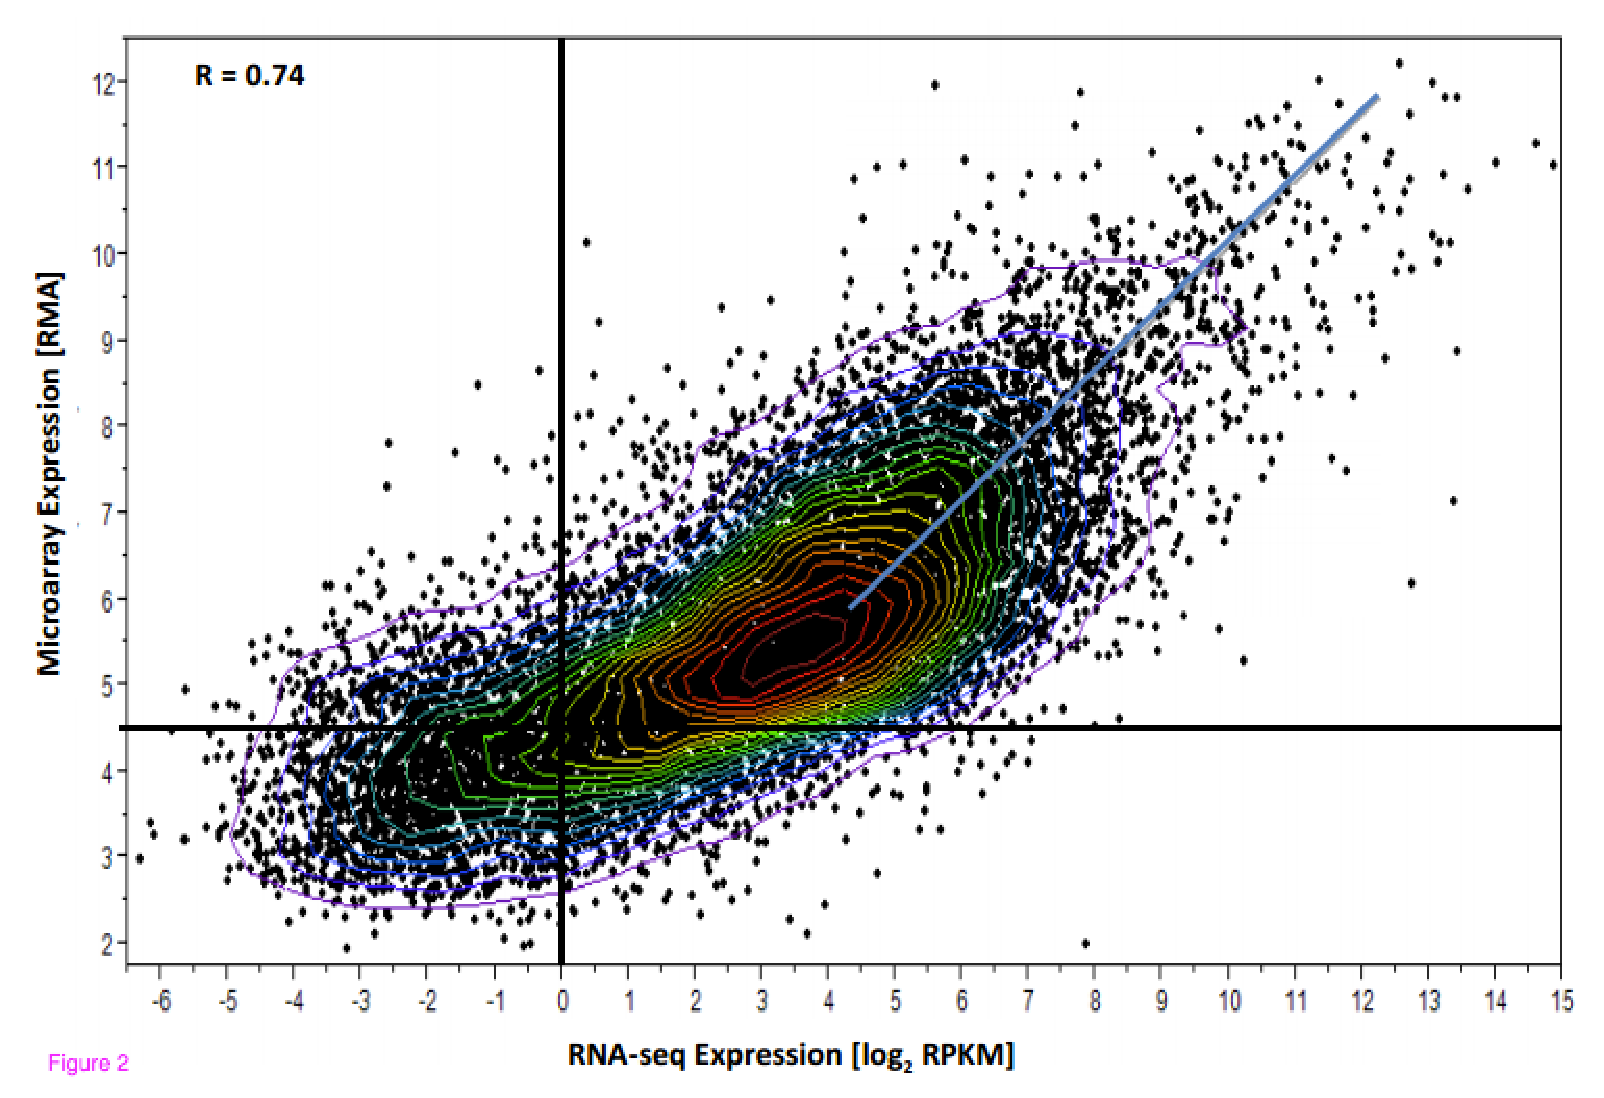
\includegraphics[width=7cm,height=6cm]{Images/Fig2.eps}
\includegraphics[width=12cm,height=6cm]{Images/photo1.eps}\\
\vspace{-0.2cm}
\caption{\footnotesize{Schematic representation of the hybrid FCNN–LSTM framework.}}\label{fig1}
\end{center}
\end{figure}


\section{Results}
The predictive performance of the proposed hybrid FCNN–LSTM framework was evaluated against several benchmark machine learning and deep learning models, including Elasticnet Regression (ELAST), Random Forest (RF), Extra Trees (EXTRA) and Light gradient boosting machine (LGBM), standalone FCNN, and standalone LSTM architectures. Hyperparameter optimization for ML models was conducted using RandomizedSearchCV. The resulting optimal hyperparameter values are reported in Table 2. Model performance was assessed using RMSE and $R^{2}$ metrics on the test dataset. In addition, to determine whether the observed performance differences between the hybrid model and the benchmark models were statistically significant, a paired (t)-test was performed on the prediction errors obtained from the same test samples. 

%The resulting (p)-values were used to assess whether the improvements achieved by the proposed model were statistically significant at the 5\% significance level.

Table \ref{tab3} presents the predictive performance of all models for PM2.5 forecasting. Among the conventional machine learning models, LGBM achieved the best performance with an RMSE of 17.1871 and an $R^{2}$  value of 0.6196, outperforming RF, Extra Trees, and Elastic Net models. The standalone FCNN and LSTM deep learning models showed comparatively weaker performance, with RMSE values of 18.8173 and 19.6636, respectively. The FCNN model was able to capture nonlinear feature relationships but lacked temporal memory, while the LSTM model effectively modeled sequential dependencies but exhibited limited capability in learning complex nonlinear feature interactions. The proposed FCNN–LSTM framework achieved the best overall performance across all evaluation metrics, obtaining the lowest MAE (11.2019) and RMSE (16.4872), together with the highest $R^{2}$ value (0.6596). Compared with standalone FCNN and LSTM models, the hybrid framework substantially reduced prediction errors and improved generalization capability. The paired $t$-test results in Table \ref{tab3} further confirm that the proposed FCNN–LSTM model significantly outperforms all benchmark models, with all comparisons yielding $p$-values below 0.05. These results indicate that integrating nonlinear feature extraction with temporal sequence modeling enables the proposed architecture to better represent the complex dynamics of air pollution data. However, the obtained R² indicates that a substantial portion of the variability in PM2.5 concentrations remains unexplained. Similarly, although the achieved RMSE and MAE values represent improvements over the benchmark models, prediction errors remain non-negligible, particularly during periods characterized by abrupt changes or extreme pollution episodes. These findings suggest that the proposed hybrid architecture provides a useful framework for PM2.5 prediction, but there remains considerable room for improvement. Future work may explore additional explanatory variables, spatial dependencies among monitoring stations, and more advanced forecasting architectures to better capture complex pollution dynamics and improve performance during extreme events.


\begin{table}[h]
\begin{center}
\small
\caption{Comparative performance of machine Learning and deep learning models}\label{tab3}
\begin{tabular}{|c|cccc|}
  \hline
  Model & MAE & RMSE& $R^{2}$& Paired $t$-test $p$-value\\  \hline \hline
  RF & 12.7296 &17.9758&0.5949& 0.006 \\
 EXTRA& 13.3518 & 18.7812 & 0.5607& $<$0.001 \\
  LGBM & 11.9912 & 17.1871 & 0.6196& 0.014  \\  
  ELAST &12.6672 & 18.1498 & 0.5870& $<$0.001  \\  
  FCNN & 13.2373 & 18.8045 &0.5461&  $<$0.001 \\  
 LSTM & 13.9852 & 19.1561 & 0.5399& 0.000 \\   
  FCNN-LSTM &11.6669 & 16.9333&0.6583 &-\\    \hline
\end{tabular}
\end{center}
\end{table}
%%%%%%%%%%%%%%%%%%%%%%%%%%%%%%% Figure %%%%%%%%%%%%%%%%%%%%%%%%%%%%%%%%%


Figure \ref{fig2} further illustrates the comparison between the observed PM2.5 concentrations and the predictions generated by FCNN, LSTM, and the proposed FCNN–LSTM framework. The standalone FCNN and LSTM models generally followed the overall trend of the target series but struggled to accurately capture abrupt fluctuations and sharp pollution peaks. The FCNN-LSTM hybrid model achieved the closest agreement with the true PM2.5 values. The model predictions more accurately tracked both short-term fluctuations and long-term trends. Although some discrepancies remain during extreme peak events, the hybrid model exhibited greater stability and lower deviation throughout the testing sequence. In particular, the hybrid model reduced prediction errors near sudden spikes and rapid transitions, indicating that combining the feature extraction capability of FCNN with the sequential learning strength of LSTM enhanced the overall forecasting performance. 
The superior behavior of the proposed framework can be attributed to the complementary roles of its components. The FCNN module extracted informative nonlinear latent representations from meteorological and pollutant variables, while the LSTM module effectively modeled temporal evolution and long-term dependencies. Consequently, the hybrid architecture achieved more stable predictions and reduced deviations from the observed pollutant concentrations, particularly during highly dynamic periods. These findings confirm the effectiveness of combining FCNN and LSTM networks within a unified framework for complex sequential prediction tasks. 

%An important characteristic of the proposed architecture is its generalized design. Unlike application-specific forecasting models, the FCNN–LSTM framework was developed as a flexible sequential prediction framework capable of handling both nonlinear feature interactions and temporal dependencies simultaneously. Although the framework was evaluated using air pollution data in this study, the proposed architecture can potentially be extended to other sequential forecasting applications such as energy demand prediction, financial time-series analysis, healthcare monitoring, and industrial process forecasting.




\begin{figure}[ht]
\begin{center}
%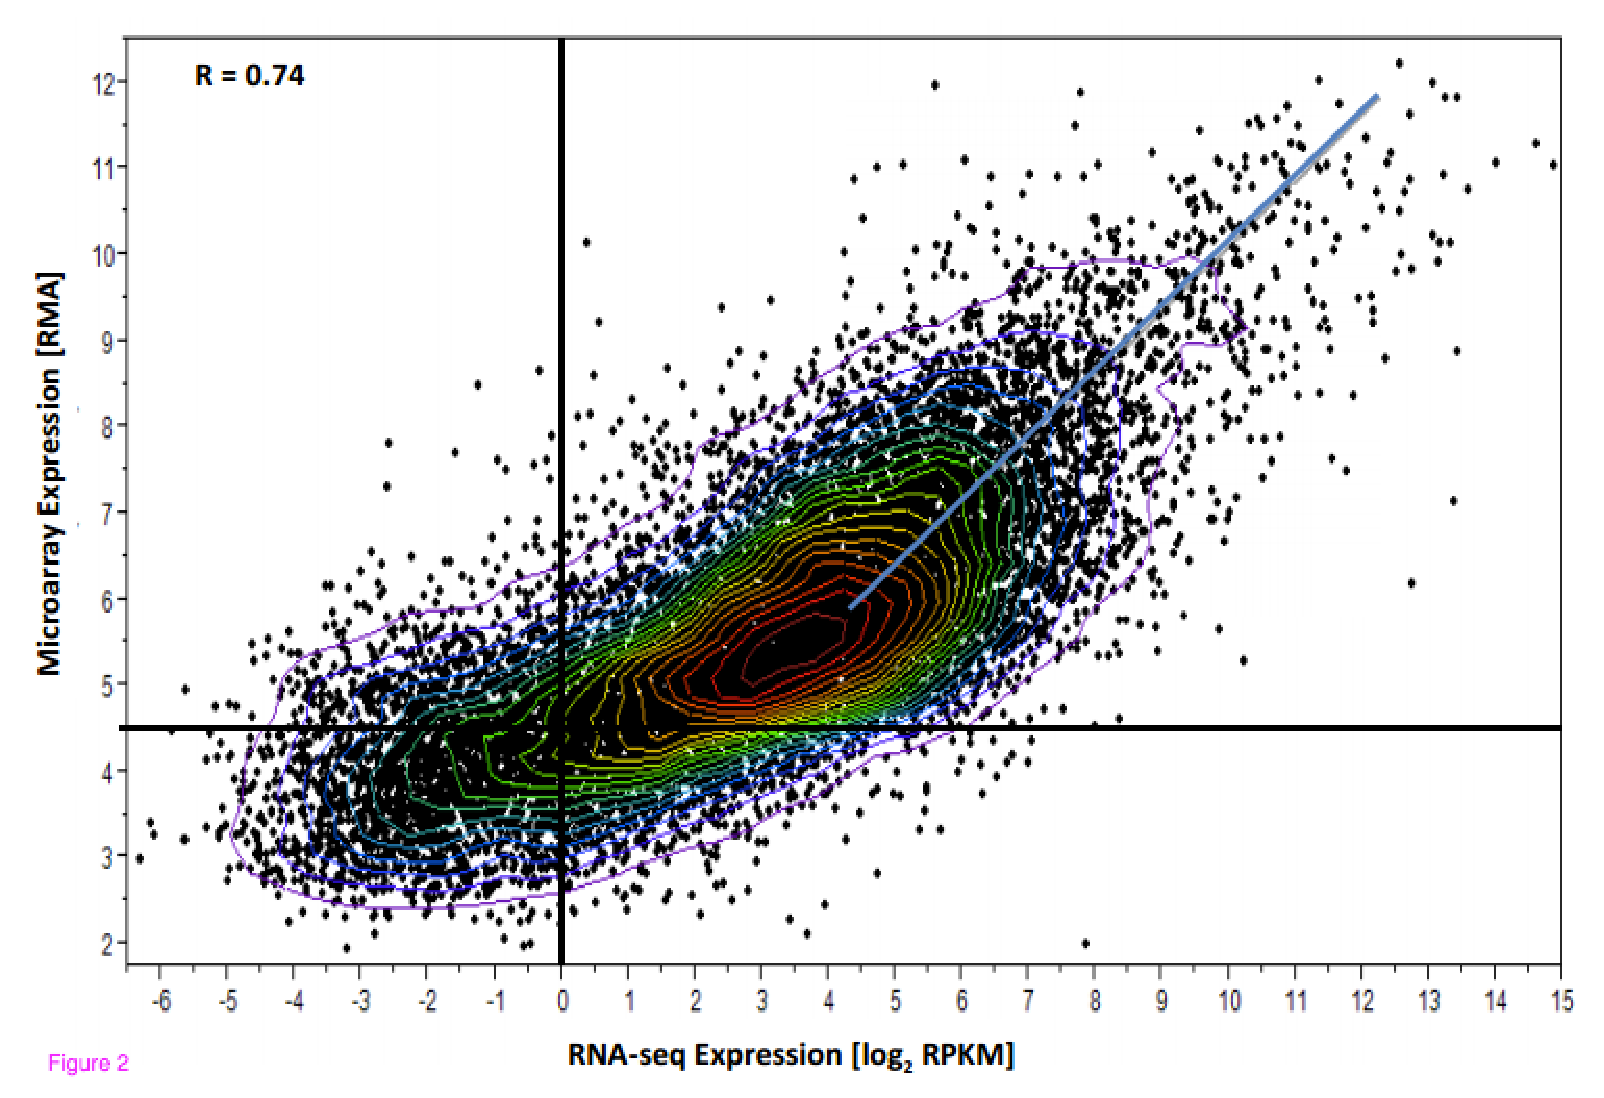
\includegraphics[width=7cm,height=6cm]{Images/Fig2.eps}
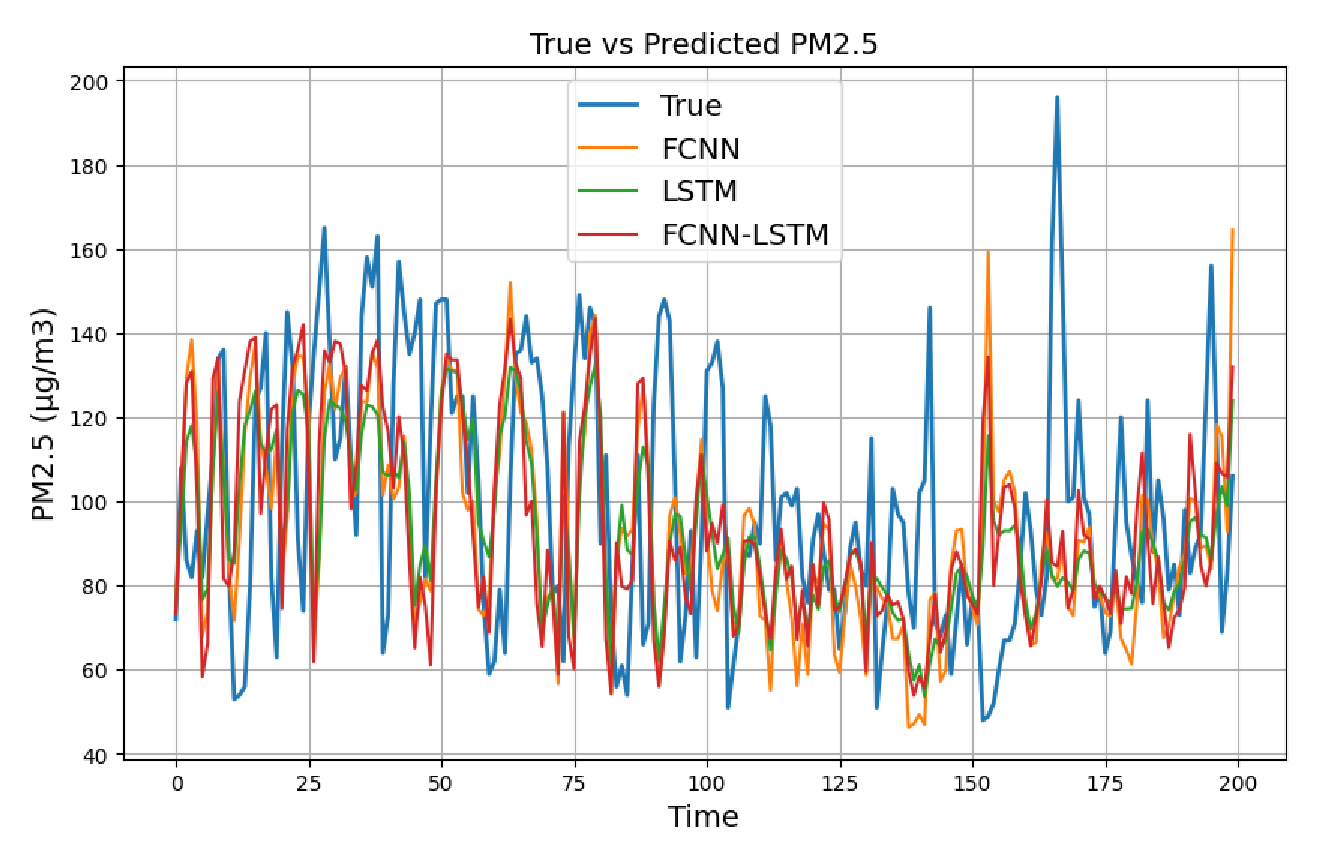
\includegraphics[width=10cm,height=5cm]{Images/Figure1.eps}\\
\vspace{-0.2cm}
\caption{\footnotesize{Temporal prediction plot for PM2.5 concentrations.}}\label{fig2}
\end{center}
\end{figure}

\section*{Conclusion}   
This study proposed a generalized hybrid FCNN–LSTM framework for sequential prediction by integrating nonlinear feature learning with temporal dependency modeling in a unified architecture. The FCNN component was designed to extract high-level nonlinear interactions among input features, while the LSTM module captured the inherent temporal dynamics and long-term dependencies present in sequential data. This complementary design enabled the model to learn both cross-sectional feature relationships and time-evolving patterns more effectively than single-architecture approaches. The experimental evaluation conducted on real-world air pollution data demonstrated that the proposed hybrid framework consistently outperformed standalone FCNN and LSTM models, as well as several conventional machine learning baselines. The improvement in predictive accuracy indicates that isolating either feature learning or temporal modeling is insufficient for complex atmospheric datasets, where pollutant concentrations are jointly influenced by nonlinear meteorological interactions and delayed temporal effects. By combining both components, the proposed model reduced prediction error and improved overall stability across different forecasting horizons. Overall, the findings confirm that integrating FCNN-based nonlinear feature extraction with LSTM-based temporal modeling leads to a more expressive and accurate forecasting framework for sequential prediction tasks. Future research will extend the comparative analysis to contemporary time-series forecasting architectures, including Temporal Convolutional Networks (TCNs), transformer-based models such as Informer and Autoformer, and graph neural network frameworks capable of exploiting spatial dependencies among monitoring stations.



%\section{How to Cite References}
%References must be cited in the text. \cite{Craik:2005}, \cite{Feller:1972}, \cite{Genest:Rivest:1993}, and \cite{LZ15} are %some examples of English references.

\section*{Acknowledgments}   
The authors gratefully acknowledge Dr. Abdullah Kaviani Rad and Dr. Mohammad Javad Nematollahi for providing the air pollution dataset utilized in this research. 
%%%%%%%%%%%%%%%%%%%%%%%% References %%%%%%%%%%%%%%%%%%%%%%%%%%%%%

\begin{thebibliography}{9}



\bibitem[Goodfellow et al. (2016)]{LZ33}
Goodfellow, I., Bengio, Y., and Courville, A. (2016). {\it Deep learning}, MIT Press.



\bibitem[Méndez et al. (2023)]{LZ1}
Méndez, M., Merayo, M.G. and Núñez, M. (2023), Machine learning algorithms to forecast air quality: a survey. {\it Artif Intell Rev}, 56, 10031–10066.

\bibitem[Pak et al. (2025)]{LZ3}
Pak, A., Rad, A.K., Nematollahi, M.J., and Mahmoudi, M., (2025), Application of the Lasso regularisation technique in mitigating overfitting in air quality prediction models. {\it Sci Rep} 15, 547. 

\bibitem[Rad et al. (2025)]{LZ13}
Rad, A.K., Nematollahi, M.J., Pak, A., and Mahmoudi, M., (2025), Predictive modeling of air quality in the Tehran megacity via deep learning techniques. {\it Sci Rep}, 15, 1367 (2025).

\bibitem[Sherstinsky (2020)]{LZ34}
Sherstinsky, A. (2020). Fundamentals of recurrent neural network (RNN) and long short-term memory (LSTM) network. {\it Physica D: Nonlinear Phenomena}, 404, 132306.


\bibitem[Wen et al. (2024)]{LZ4}
Wen, X., Liao, J., Niu, Q.  Nachuan Shen, N., Yingxu Bao, Y., (2024), Deep learning-driven hybrid model for short-term load forecasting and smart grid information management. {\it Sci Rep}, 14, 13720.

\bibitem[Zhang et al. (2022)]{LZ2}
Zhang, B., Rong, Y., Yong, R., Qin, D.,  Li, M., Zou, G., Pan, J., (2022), Deep learning for air pollutant concentration prediction: A review. {\it Atmospheric Environment}, 290, 119347.





\end{thebibliography}
 \end{document}

